\chapter{Vorarbeit}

Dieses Kapitel befasst sich mit der \ac{SNP} Annotation im allgemeinen, zusätzlich wird die Vorarbeit zu dieser Arbeit kurz vorgestellt.




\section{Einzelnukleotid-Polymorphismus}
Bevor auf die Annotation der \ac{SNPs} eingegangen werden kann, muss erst der Begriff des Einzelnukleotid-Polymorphismus erklärt werden. Dieser kommt aus dem englischen \emph{Single Nucleotide Polymorphism} (SNP) und in wird in dieser Arbeit auch nur unter diesem Namen verwendet.

Ein \ac{SNP} ist eine genetische Variation einer Base im Genom, dies bedeutet, dass eine Base im Beispiel Abb. \ref{fig:snp} Adenin durch Thymin ausgetauscht wurde.

\begin{figure}
\centering
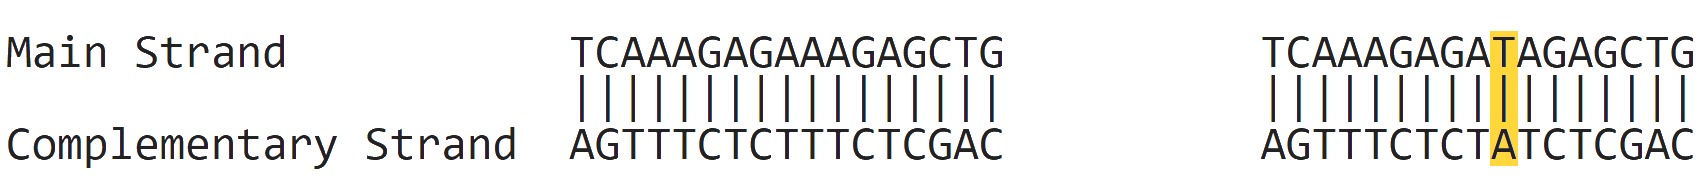
\includegraphics[width=.95\textwidth]{images/DNA_ds_strand_with_snp.png}
\caption{Doppelsträngiger DNA Ausschnitt der ABL proto-oncogene 1 tyrosine kinase mit \ac{SNP} (gelb hervorgehoben) rechts und ohne links.}
\label{fig:snp}
\end{figure}

%\begin{lstlisting}
%Main Strand           TCAAAGAGAAAGAGCTG          TCAAAGAGATAGAGCTG
%                      |||||||||||||||||          |||||||||||||||||
%Complementary Strand  AGTTTCTCTTTCTCGAC          AGTTTCTCTATCTCGAC
%\end{lstlisting}


Durch \emph{whole genome} \ac{SNP} Analysen wurde ermittelt, dass genetische Variationen zwischen menschlichen Genomen fast gänzlich durch \ac{SNPs} dargestellt werden \cite{Do.2015}. 
\ac{SNPs} können in \emph{open reading frames} (orf), aber auch in nicht codierenden Bereichen der DNA vorkommen. Einige \ac{SNPs} liegen direkt in Exons und werden in Protein translatiert. Diese Proteine können, je nach Art des \ac{SNPs}, eine veränderte Struktur und Funtktion aufweisen. Jedoch können auch nicht kodierende \ac{SNPs} das Risiko für bestimmte Erkrankungen erhöhen, z.B. beeinflussen einzelne \emph{non coding} \ac{SNPs} im Gen \emph{IKZF1} das Risiko für Kinder an ALL zu erkranken \cite{Papaemmanuil.2009}.

Es gibt verschiedene Arten von \ac{SNPs}:

\begin{description}
\item[Frameshift]
Ein \emph{Frameshift} sorgt durch eine \emph{Insertion} oder \emph{Deletion} für eine Verschiebung des Leserasters und ist fast immer pathogen.
\item[Missense]
Der häufigste Typ der \ac{SNPs} ist die sogenannte \emph{Missense variation}, hierbei wird eine Base durch eine andere ausgetauscht und ggf. auch die entstehende Aminosäure verändert, wenn sich der \ac{SNP} in einem codierenden Bereich befindet. 
\item[Nonsense]
Die \emph{Nonesense} Mutation sorgt für eine Entstehung eines termininierende Triplets, welches die Transkription vorzeitig abbricht.
\item[Splice site]
Ist ein SPN in einer \emph{splicing site}, so können einige Transkripte des Gens von dem \ac{SNP} verändert werden, während Andere nicht beeinflusst werden.
\item[ncRNA]
Wie oben erwähnt gibt es \emph{non coding} (nc) Bereiche in denen \ac{SNPs} liegen können, liegt nun ein \ac{SNP} in einem Intron, so wird es durch den Splicing Prozess herausgeschnitten und letztendlich nicht in Protein translatiert. 
\item[Near gene]
Eine weitere Besonderheit sind SNPs, welche sich in der Nähe von Genen aufhalten. Somit sollten diese nach bisherigem Wissen keinen Einfluss auf den Organismus haben, jedoch wurde gezeigt, dass es epigenetische Faktoren gibt, wie \emph{Silencer} Regionen, welche so die Expression eines Gens beeinflussen können\cite{Maston.2006}. 
\item[UTR]
UTR steht für \emph{untranslated regions} und bezeichnet den Bereich, welcher innerhalb der mRNA vor dem Start- und hinter dem Stoppcodon liegt also jenen, welcher nicht in eine Aminosäuresequenz translatiert wird.
\end{description}

\textbf{Soll ich noch eine Abbildung machen, welche exemplarisch alle \ac{SNP} Arten zeigt?}



\section{SNP Annotation}
\begin{sloppypar}
Um zu verstehen welche Auswirkungen ein \ac{SNP} auf den Organismus hat, ist es wichtig diesen zu annotieren. 
Für die Annotation von \ac{SNPs} existieren derzeit über 20 verschiedene verschiedene Algorithmen zur funktionellen Vorhersage: \texttt{SIFT}, \texttt{Polyphen2-HDIV}, \texttt{Polyphen2-HVAR}, \texttt{LRT}, \texttt{MutationTaster2}, \texttt{MutationAssessor}, \texttt{FATHMM}, \texttt{MetaSVM}, \texttt{MetaLR}, \texttt{CADD}, \texttt{VEST3}, \texttt{PROVEAN}, \texttt{FATHMM-MKL coding}, \texttt{fitCons}, \texttt{DANN}, \texttt{GenoCanyon}, \texttt{Eigen coding}, \texttt{Eigen-PC}, \texttt{M-CAP}, \texttt{REVEL}, \texttt{MutPred}. 
\end{sloppypar}
Außerdem gibt es noch Algorithmen, welche den Grad der Konservierung einer Position analysieren, dazu zählen: \texttt{PhyloP, phastCons, GERP++} und \texttt{SiPhy}.

Alle Algorithmen in dieser Arbeit vorzustellen wäre nicht zielführend und würde den Rahmen sprengen. Daher wird in dieser Arbeit nur auf die wichtigsten Unterschiede zwischen den Algorithmen exemplarisch eingegangen. 

\begin{figure}
\centering
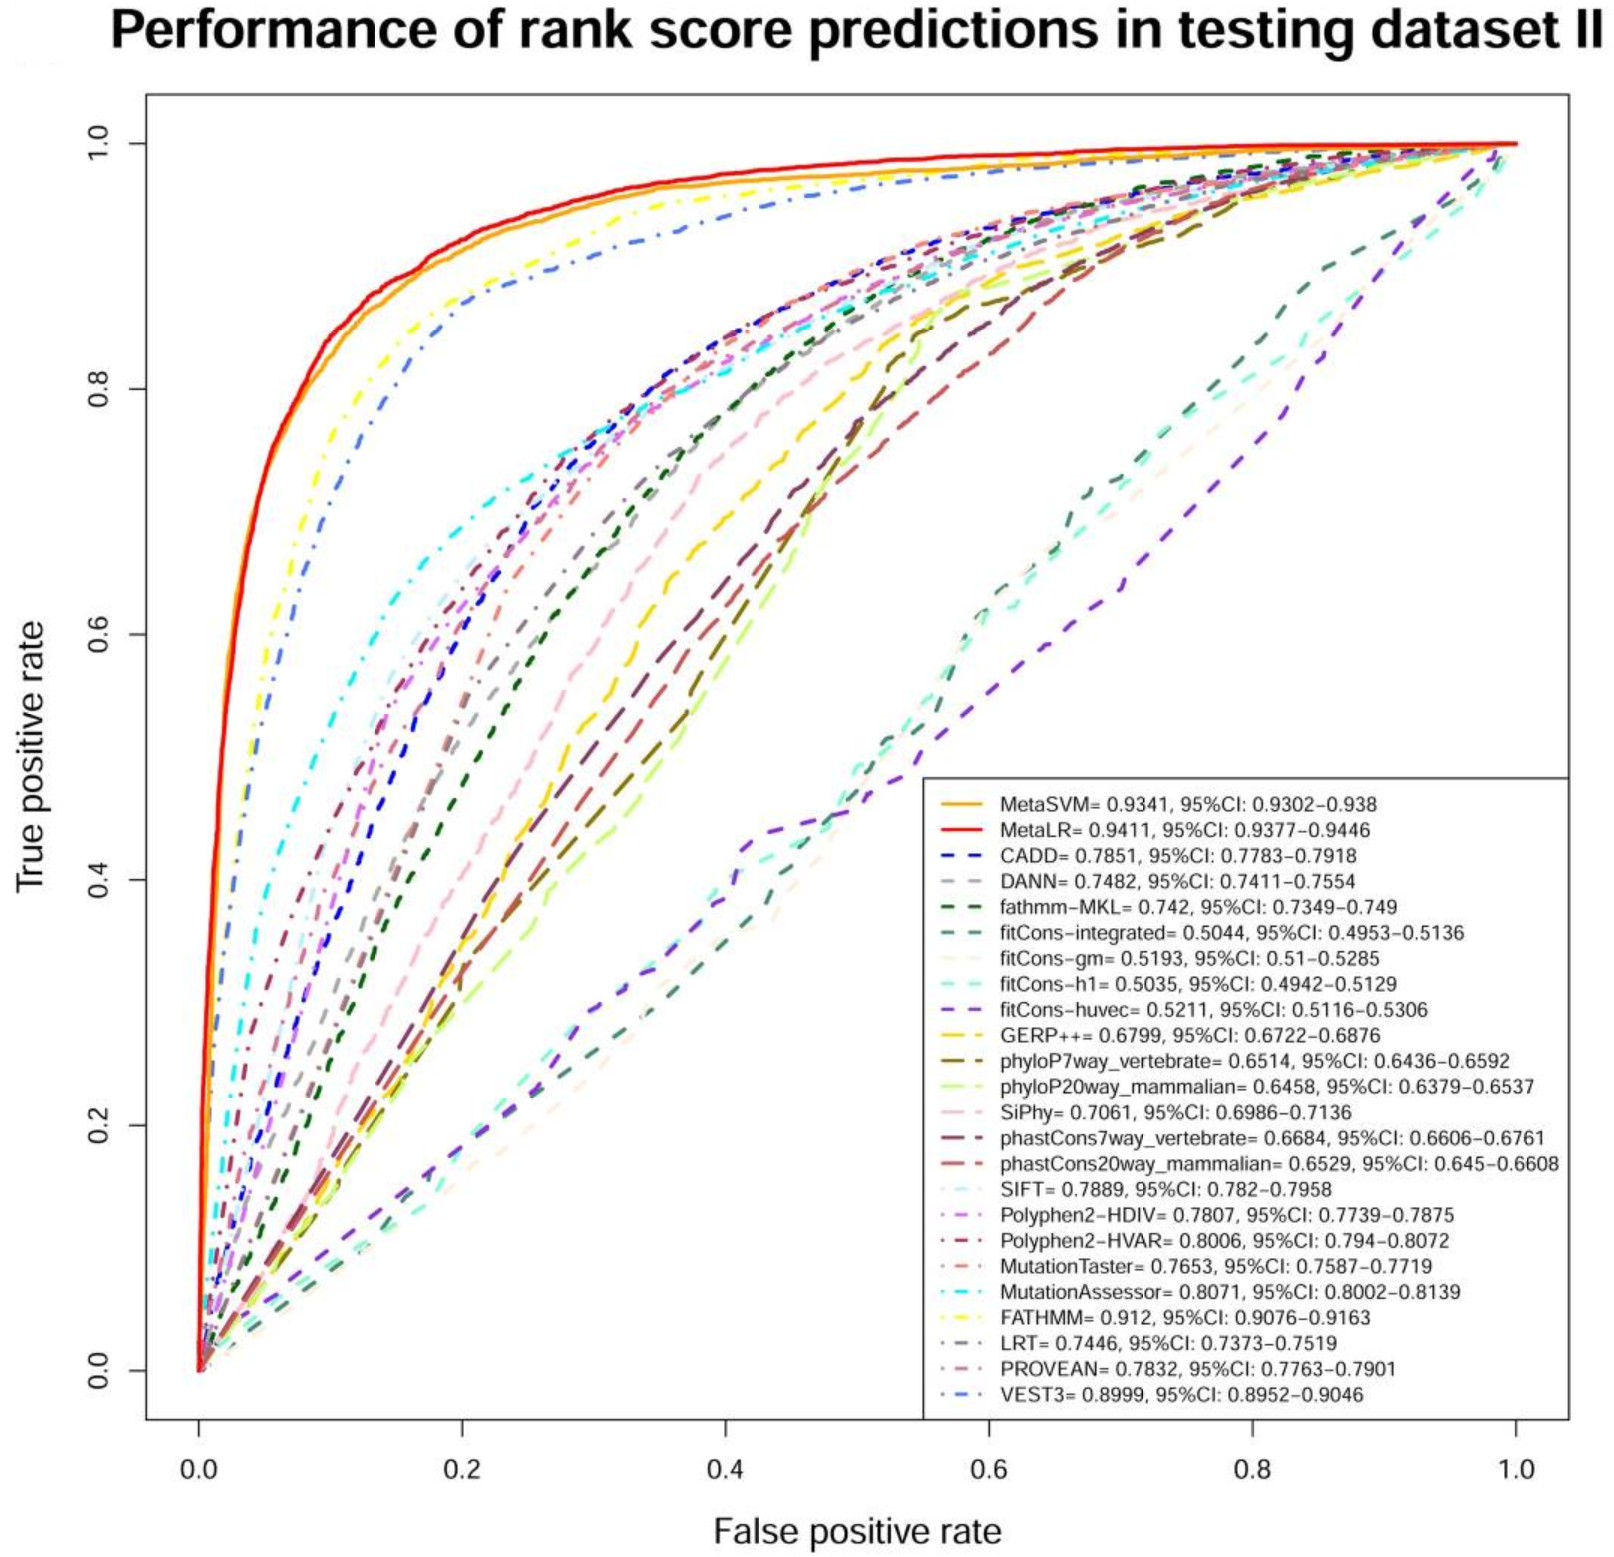
\includegraphics[width=.95\textwidth]{images/compared_prediction_scores.png}
\caption{\ac{ROC} Kurven für die funktionellen Vorhersage- und Konservierungs- Scores der dbNSFP v3.0 mit Testdatensatz II aus\cite{Liu.2016}}
\label{fig:comp_scores}
\end{figure}

So arbeitet der \texttt{Sift}\cite{Vaser.2016} Algorithmus mit der Wahrscheinlichkeit mit der eine Aminosäure an einer Position toleriert wird, anhand von Referenz Protein Familien.
\texttt{Polyphen2}\cite{Adzhubei.2013} steht für \emph{Polymorphism phenotyping}, dieser Algorithmus arbeitet mit \emph{machine learning} und einem Trainingsdatenset \emph{HumDiv/HumVar}.
\texttt{FATHMM}\cite{Shihab.2013} steht für \emph{Functional Analysis through Hidden Markov Models} und arbeitet wie der Name schon sagt mit Hidden Markov Modellen.
Als letztes ist noch der \texttt{DANN} \cite{Quang.2015} Algorithmus erwähnenswert, dieser Arbeitet mit neuronalen Netzwerken, was auch sich auch in seinem Namen wiederspiegelt: \emph{deleterious annotation of genetic variants using neural networks}.

Hierbei ist wichtig zu erwähnen das kein Algorithmus eine perfekte Vorhersage treffen kann. So wurde in der Arbeit \cite{Liu.2016} ein Trainingsdatensatz bekannter SNPs mit allen Algorithmen annotiert und das Ergebnis ausgewertet siehe \ac{Abb} \ref{fig:comp_scores}. Hierbei lieferte MetaSVM eine \ac{SVM} und MetaLR eine \ac{LR} über alle Scores, also eine Kombination aus allen Scores das beste Ergebnis.

%https://www.ncbi.nlm.nih.gov/pmc/articles/PMC4752381/ 

Zusätzlich gibt es noch eine unbestimmte Anzahl von Weiterentwicklungen und Variationen der etablierten Vorhersage Algorithmen, wie z.B. der neue \texttt{FATHMM-XF}\cite{Rogers.2017} oder \texttt{SIFT-MS}\cite{Smith.2015}.



\section{SNP annotation programm for AML}
\label{sec:sapa}
In einer vorherigen Arbeit wurde ein Programm namens \emph{SAPA}\footnote{\url{https://github.com/TobiasJu/SAPA}} erstellt, welches zur Annotation von \emph{Illumina truseq amplicon variants} Daten dient. Das Programm nutzt die oben erwähnten Algorithmen, allerdings aus Performancegründen nicht alle explizit, sondern nutzt die dbNSFP\cite{Liu.2016}, indem als Backend auf Annovar\cite{Wang.2010} gesetzt wird. 

Das Programm wurde am Ende mit einem Clinvar Datensatz aus 2023 pathogenen und 2000 benignen \ac{SNPs} getestet. Bei den Daten handelt es sich ausschließlich um \ac{SNPs} welche von mehreren Autoren die gleiche Vorhersage erhalten haben. Somit sollte die bestmögliche Konsistenz gewährt sein.

Nach der Auswertung der Annotation wurde so ein \emph{MCC} von 0,64 ermittelt.